\documentclass[11pt,a4paper]{article}
\usepackage[margin=20mm]{geometry}
\usepackage{fontspec,xeCJK}
\setmainfont{TeX Gyre Termes}
\setsansfont{TeX Gyre Heros}
\setmonofont{DejaVu Sans Mono}[Scale=0.8]
\setCJKmainfont{Noto Serif CJK TC}
\setCJKsansfont{Noto Sans CJK TC}
\setCJKmonofont{Noto Sans Mono CJK TC}
\usepackage{amsmath,amssymb,booktabs,tabularx,graphicx,xcolor,enumitem,float}
\usepackage[unicode,colorlinks=true,linkcolor=blue!50!black,urlcolor=blue!50!black,citecolor=blue!50!black]{hyperref}
\usepackage{fancyhdr}
\pagestyle{fancy}\fancyhf{}
\fancyhead[L]{\small ML2026@IAII — Regression}
\fancyhead[R]{\small 314580075 黃駿甯}
\fancyfoot[C]{\thepage}
\setlength{\headheight}{15pt}
\setlength{\parindent}{0pt}
\setlength{\parskip}{5pt}
\setlist{nosep,leftmargin=1.6em}
\emergencystretch=2em
\title{314580075｜ML2026@IAII -- Regression\\Kaggle 1 Competition\\\large 台灣住宅成交總價預測\\時間泛化、非價格地理特徵與學習式政策住宅分支}
\author{黃駿甯（學號 314580075）\\\small snoopyjim · \href{mailto:adogg5528@gmail.com}{adogg5528@gmail.com}}
\date{2026 年 10 月 31 日}

\begin{document}
\maketitle
\begin{abstract}
本專案針對 ML2026@IAII 台灣房價競賽，以原始新臺幣總價的平均絕對誤差（MAE）評估。
方法由面積尺度與時間行情特徵、CatBoost／LightGBM 集成、非價格道路位置特徵，以及學習式安置住宅分支組成。
最終候選 v7 的使用者回報 public MAE 為 \textbf{1,716,414.5323 元}，相對 v6 改善 1.66\%。
在三個一年期歷史窗口，一般住宅地理增量的整體 MAE 分別改善 1.99\%、1.72\%、2.85\%。
外部政策分支先排除所有 test 同戶報價，再用其他 441 戶學習物理特徵與房地報價的關係。
額外整基地留出及相似樣本排除測試支持同政策制度內的泛化，但不代表已驗證實際成交價或其他安置制度。
本報告保留失敗候選、驗證重用與外部來源時間限制，不宣稱零過擬合、private 最佳或已取得第一名。
\end{abstract}

\section{任務、資料與評估}
對每筆 test 交易預測 \(\hat y_i\)，輸出兩欄 \texttt{編號,總價元}。官方指標為
\begin{equation}
\mathrm{MAE}=\frac{1}{n}\sum_{i=1}^{n}|y_i-\hat y_i|.
\end{equation}
本專案最初曾比較對數尺度與平方誤差方法，確認競賽指標後，正式候選選擇均使用原價 MAE。
對數損失仍可作為部分模型的訓練替代目標，但不取代正式評估指標。

原始 train 為 455,787 列，移除 3 列英文欄位說明及 8 列日期無效或超出訓練範圍的資料，保留 455,776 列。
沒有依總價高低刪除交易。官方 valid 為 11,994 列，test 為 47,073 列。
train 的有效日期截至 2024-08-10；test 日期介於 2024-08-11 與 2025-07-31。
官方 valid 的分布較接近舊訓練資料，因此低 valid 誤差不等於能預測未來一年。

輸入包含行政區、地址、土地／建物／車位面積、交易日期、樓層、建物型態、用途、建材、格局、管理、車位、備註與建案等欄位。
建築完成年月在原 train 幾乎不可用，沒有假造可靠屋齡。
ID 只用於輸出對齊；一般房價特徵不直接使用目標價格或備註金額。
安置住宅備註的明列減收差額另作可追溯的帳務運算。

\section{模型架構}
\subsection{面積、時間與表格模型}
基礎特徵涵蓋淨面積、面積比、每房面積、樓層占比、頂樓／一樓、房廳衛、車位數與語義旗標。
地址解析產生城市、行政區、道路、路口、地段與正規化建案鍵；字元 TF--IDF／SVD 表示只在當折 fitting 地址上擬合。
訓練資料內的歷史行情及同建案價格趨勢用於時間調整，validation／test 標籤不參與估計。

對有效面積 \(A_i\) 與從 fitting 資料估計的時間因子 \(I_i\)，部分分支學習
\begin{equation}
z_i=\log\frac{y_i}{A_i I_i},\qquad
\hat y_i=A_i I_i\exp(f(x_i)),
\end{equation}
並以已凍結的趨勢衰減控制未來外推。其他分支學習總價或單價，以降低對單一尺度假設的依賴。
若單價 L1 的樣本權重為面積，則
\(A_i|y_i/A_i-f(x_i)|=|y_i-A_i f(x_i)|\)，
可在單價表達下對齊總價 MAE。不是所有分支都採用此損失；地理 CatBoost 使用加權對數 RMSE，再以原價 MAE 決定是否採用。

一般住宅基準逐輪保留既有集成，再加入經跨年度檢驗的候選。
v4 的已見建案部分採用 v3 與新的 LightGBM 分支各半；未見建案沿用 v3。
v6 僅替換安置住宅分支，其餘價格沿用 v4。

\subsection{非價格地理增量（v7）}
使用警政署 2020 年歷史事故資料中的\textbf{地址與經緯度}建立位置參考\cite{npa}。
此來源不包含住宅價格；沒有以外部成交價、配售價或同戶價格標籤回填一般住宅。
2020 A2 資料清理後保留 360,521 筆；A1 只用來檢查位置估計誤差。

依城市、行政區、道路、百號門牌區段及路口，估計座標中位數、參考點數與位置分散度。
新增 13 個數值特徵，包括近似經緯度、定位層級、支持度、距城市／行政區參考中心距離與附近參考點密度。
這些參考中心不是官方行政區中心；密度也不是交通可達性或事故風險的直接量測。
train／test 的道路或更細層級涵蓋率為 66.39\%／70.98\%。

對照實驗包含有／無地理特徵的 CatBoost 與 LightGBM。
CatBoost 固定深度 8、3,000 輪、學習率 0.045、L2 係數 10；兩個 seed 為 20261017、20261018。
候選只比較預定的 25\%／50\% 混合權重。最終選定地理 CatBoost 的 50\% 增量：
\begin{equation}
\hat y^{(7)}_i=
\begin{cases}
0.5\hat y^{(6)}_i+0.5\,\mathrm{mean}_{s=1,2}(\hat y^{geo,s}_i), & i\in\mathcal C,\\
\hat y^{(6)}_i,&i\notin\mathcal C.
\end{cases}
\end{equation}
\(\mathcal C\) 要求原始建案名稱與正規化建案鍵都未出現在 fitting，並排除安置住宅。
test 有 28,374 筆符合此條件；其餘 18,699 筆完全不變，包含 1,408 筆安置住宅。

\subsection{學習式安置住宅分支}
train 沒有安置住宅對應交易，test 卻有 1,408 筆。
正式分支從公開手冊的 1,845 戶房地報價中，\textbf{先排除 test 的 1,404 個同戶身分}，只用剩餘 441 戶、10 個基地訓練。
建案與棟號只用於同戶排除及分組驗證，不是價格模型輸入。
最終模型為正則化中位數回歸（L1 懲罰 \(\alpha=0.001\)），六個特徵為面積、樓層、樓層平方、一樓、二樓與露臺旗標。

交易總價組合為
\begin{equation}
\hat P=A\,\hat u(A,F,F^2,I_1,I_2,T)+N_{park}\,\hat c_{park}-D_{note}.
\end{equation}
車位常數由 2,090 筆公開車位報價估計中位數，為每位 950,000 元。
\(D_{note}\) 僅是備註明列的「原房屋價款減去減收後房屋價款」，不是模型學到的係數。
舊手冊依已公開政策統一到同一價格版本，也是前處理規則，不是因果效果估計。

曾有 v5 逐戶報價查表實驗；在使用者要求「外部資料必須用於學習、不能直接查答案」後，v5 已淘汰。
v6/v7 的推論只依物理特徵與保存模型，不讀逐戶價格表。
但研究歷程先前曾接觸這些報價，因此不宣稱整個研究從未看過被排除戶的外部報價。

\section{驗證設計與選模}
\begin{table}[H]\centering\small
\begin{tabular}{llll}
\toprule
窗口 & fitting 截止 & 未來評估期間 & 本輪角色\\
\midrule
Stress 2021 & 2021-08-10 & 2021-08-11 -- 2022-08-10 & 選模壓力檢查\\
Development & 2022-08-10 & 2022-08-11 -- 2023-08-10 & 選模\\
Confirmation & 2023-08-10 & 2023-08-11 -- 2024-08-10 & 凍結後確認\\
\bottomrule
\end{tabular}
\caption{前向時間窗口。這些窗口曾被前期研究使用，並非全新獨立測試。}
\end{table}

採用地理候選前，要求前兩個年度未見建案 MAE 各改善至少 0.5\%，後八個月不退步，且勝過相同權重的無地理特徵對照。
先凍結候選與權重，再檢查第二 seed；兩 seed 均須改善，平均仍須通過門檻。
第三年度維持同一選擇，要求改善至少 0.5\%、後八個月不退步，且建案群組 bootstrap 改善區間下界為正。
這些門檻限制當輪搜尋，但不能消除多輪重用歷史驗證的選模偏誤\cite{cawley}。

政策分支原始評估採外層五折整基地留出、內層三折選模。
候選為單價中位數、正則化中位數回歸與淺層 L1 樹。
外層房地報價 MAE 為 274,038 元，基準 302,285 元；該結果不是實際成交總價 MAE。

\section{實驗結果}
\subsection{公開成績與候選選擇}
\begin{table}[H]\centering
\begin{tabular}{lrl}
\toprule
版本 & Public MAE（元） & 狀態／差異\\
\midrule
原版 & 2,393,304.6257 & 原價 MAE 校準\\
v2 & 2,188,394.3386 & 一年期回測與表徵\\
v3 & 2,092,770.8572 & 跨年度結構模型集成\\
v4 & 2,043,963.0611 & 已見建案增量\\
v5 & 1,739,081.1170 & \textbf{逐戶查表對照，已淘汰}\\
v6 & 1,745,458.0575 & 學習式政策分支；備選\\
v7 & \textbf{1,716,414.5323} & 非價格地理增量；主選\\
\bottomrule
\end{tabular}
\caption{使用者截至 2026-10-18 回報的成績。未獨立取得官方評分紀錄；private 未知。}
\end{table}
v7 相對 v6 降低 29,043.5252 元（1.66\%）。若可保留兩份候選，選擇 v7 與 v6，分散地理增量在 private 不同區域組成下的風險。
兩者安置住宅價格完全相同，因此不能分散政策分支的共同誤差。

\subsection{同切分歷史比較}
\begin{table}[H]\centering
\begin{tabular}{lrrrr}
\toprule
年度 & 基準整體 MAE & v7 方法 MAE & 整體改善 & 未見建案改善\\
\midrule
2021--2022 & 2,267,217 & 2,222,048 & 1.99\% & 2.15\%\\
2022--2023 & 1,308,238 & 1,285,717 & 1.72\% & 2.11\%\\
2023--2024 & 1,440,869 & 1,399,774 & 2.85\% & 3.75\%\\
\bottomrule
\end{tabular}
\caption{原價 MAE，單位為元。歷史資料沒有安置住宅成交標籤，不能藉此評估政策分支。}
\end{table}
第三年度後八個月的未見建案改善 3.72\%。原凍結候選的建案群組 bootstrap 改善 95\% 區間為 36,545--107,179 元；相對無地理特徵對照為 34,361--101,527 元。
區間沒有校正全部歷史模型搜尋，也不是未來市場變化的保證。

未採用結果一併保存。建案身分遮蔽的八個候選未通過跨年度門檻；地理 LightGBM 亦未通過採用門檻。
沒有因候選失敗而放寬門檻或依 public 分數調整特定建案價格。

\section{過擬合診斷}
重新載入三年度、有／無地理特徵、兩個 seed，共 12 個模型，在 500、1,000、1,500、2,000、2,500、3,000 棵樹重算推論。
每年度使用 50,000 筆固定訓練樣本及全部未來驗證資料。
三年度地理集成的未見建案 MAE 在六個檢查點均下降，沒有觀察到該範圍內的整體後期反彈。
保存的 3,000 棵樹預測與原紀錄一致。

\begin{figure}[H]\centering
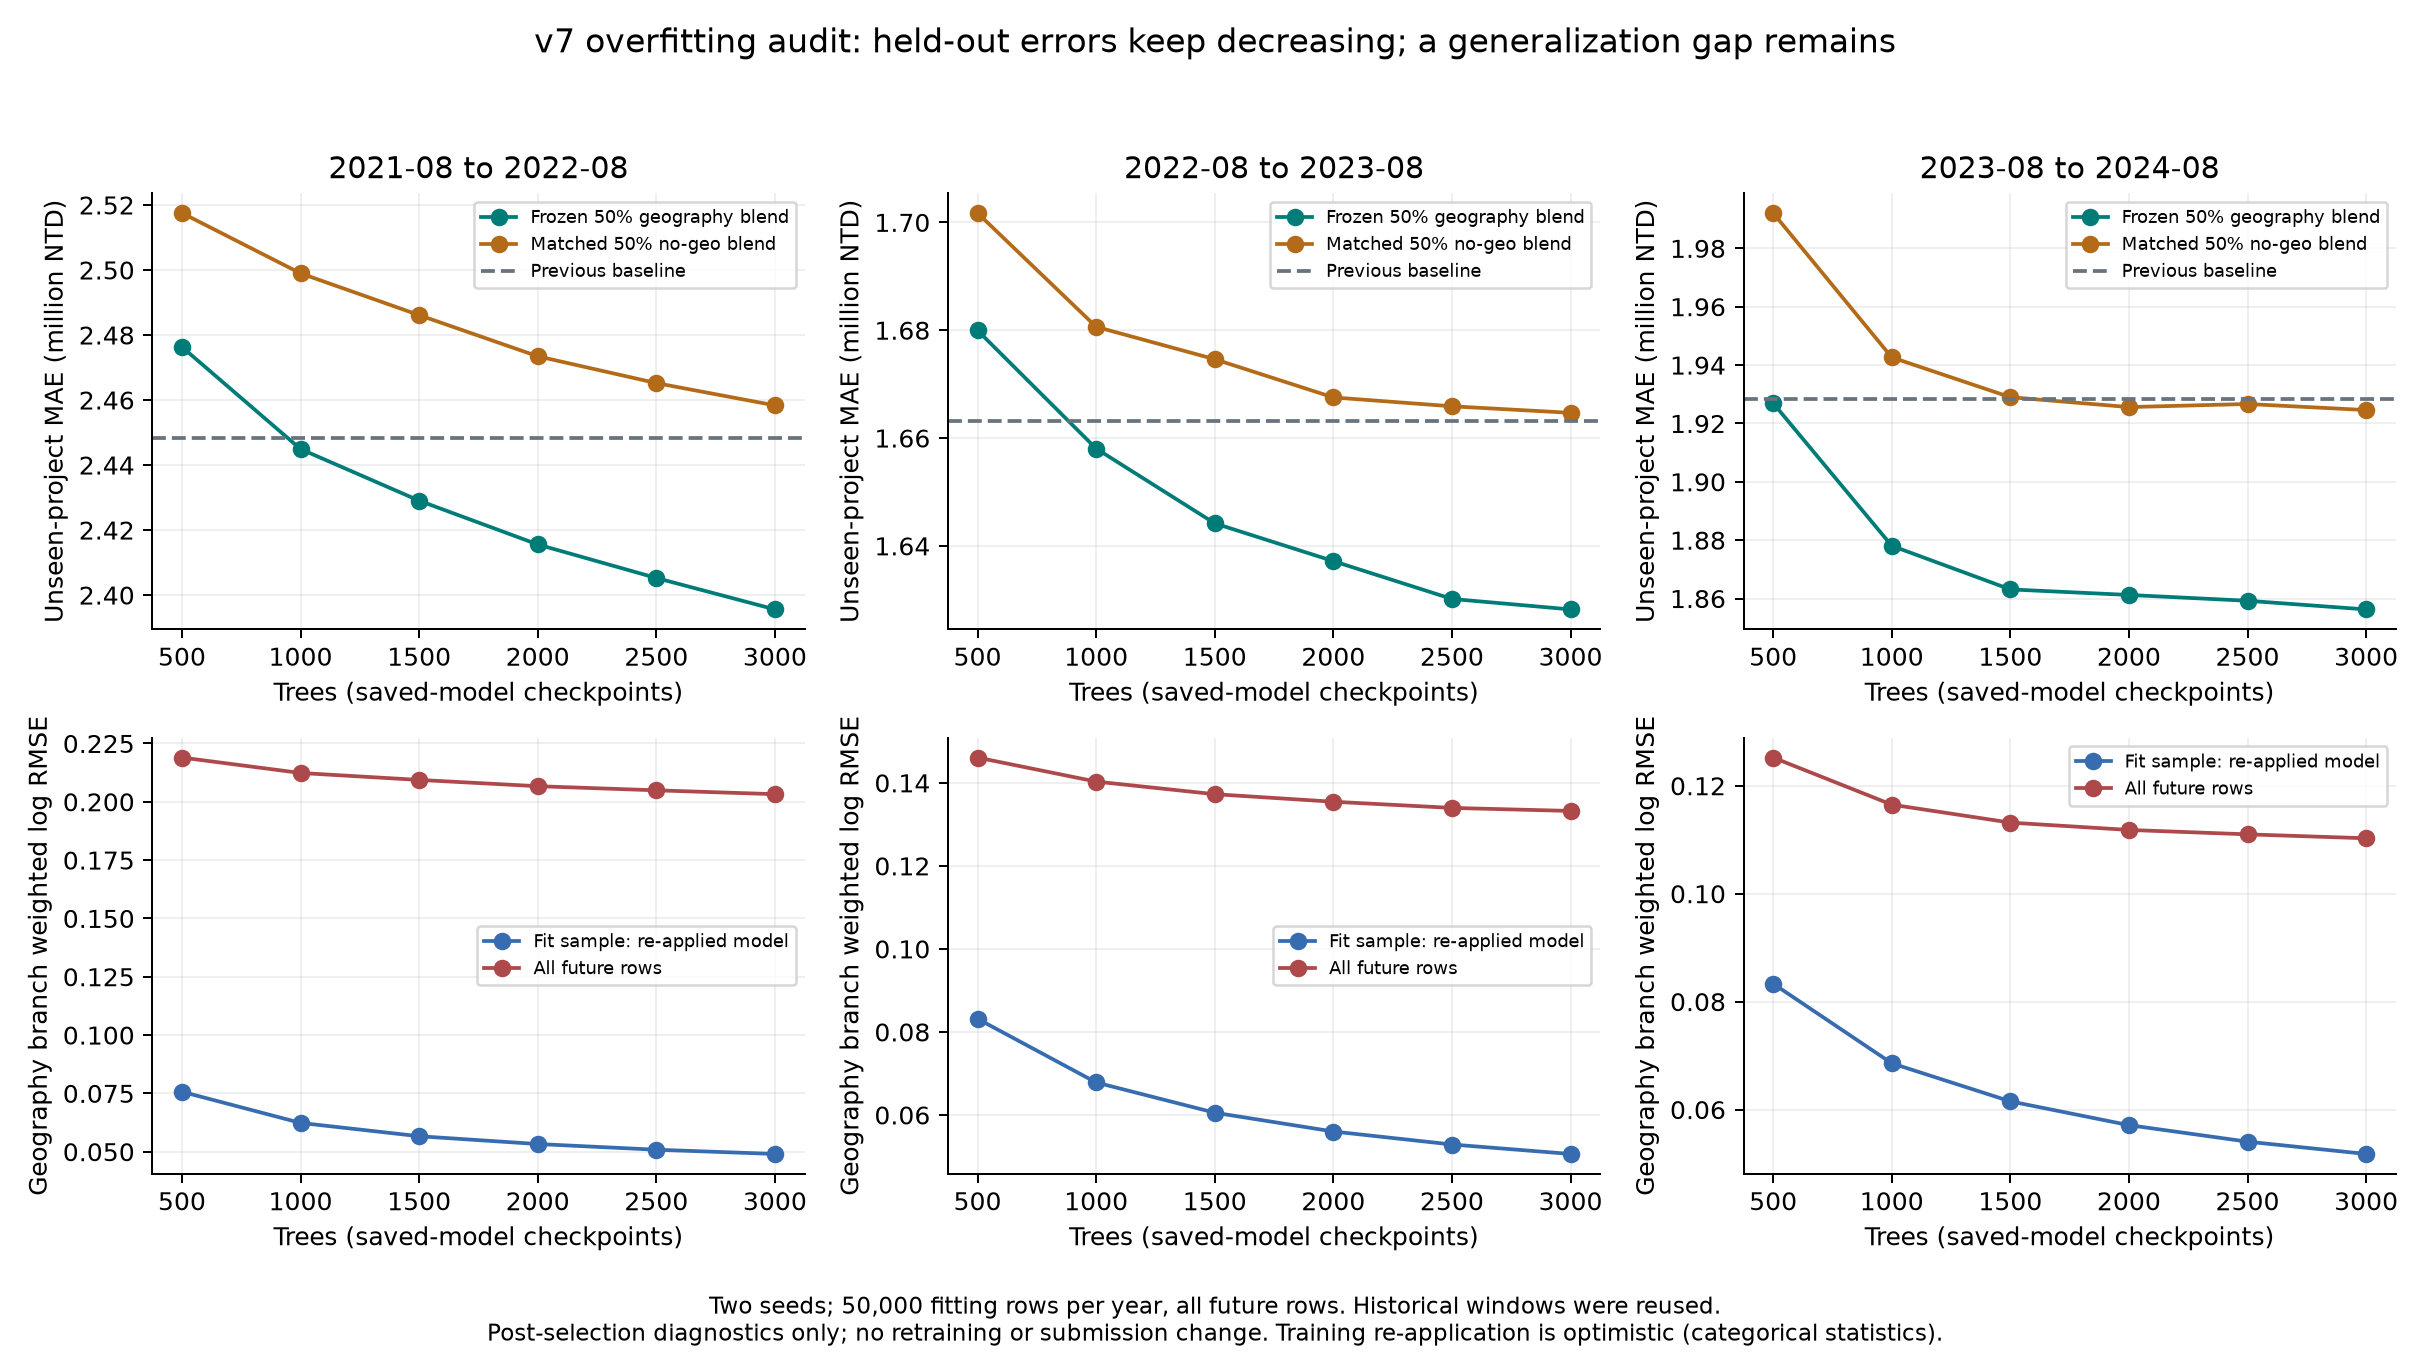
\includegraphics[width=\textwidth]{figures/overfitting.png}
\caption{上排為未見建案 MAE；下排為地理分支加權 log-RMSE。訓練／未來誤差仍有落差。}
\end{figure}

地理分支的未來資料加權 log-RMSE 約為訓練重推樣本的 2.13--4.14 倍。
市場漂移、未見建案與 CatBoost 訓練／推論時類別統計差異均可能影響此落差\cite{catboostfaq}；不能全歸因於過擬合。
各年度約 45\% 的未見建案退步；2021 年每建案等權 MAE 略差，而逐交易 MAE 改善。
排除改善總額最大的十個建案後，各年度仍改善 1.20\%、0.50\%、1.84\%，顯示增益不是完全由少數建案貢獻。
但 2022 年按城市重抽樣的改善區間包含零，區域組成改變仍是風險。

\section{安置住宅是否具泛化性}
\subsection{不依賴同戶答案的檢查}
對全部 1,408 筆實際查詢，移除／替換地址、建案、棟號、ID、任意新增價格欄，預測完全相同。
改變列順序、批次大小及重複查詢亦不改變結果。
模型載入後封鎖檔案讀取，仍能完成推論。
把被排除戶的身分拼上合成極端價格，安全訓練資料仍保持相同，並可重現原模型；未使用被排除戶真實價格作驗證。

\subsection{額外分組壓力測試}
僅以原 441 戶安全標籤作追加研究。
除了整基地留出，將相關的 A18 三期合併為同組，並測試整份來源手冊留出。
最後在基地留出後，再排除 fitting 中與驗證戶同樓層、同露臺且面積差不超過 1 m\(^2\) 的樣本。
整組留出用來避免相關群組同時落入 fitting 與 validation\cite{logo}。

\begin{table}[H]\centering\small
\begin{tabular}{lrrr}
\toprule
測試 & 基準報價 MAE & 模型報價 MAE & 改善\\
\midrule
整基地留出（10 折） & 293,780 & 243,592 & 17.08\%\\
A18 三期合併（8 折） & 293,811 & 243,835 & 17.01\%\\
整份手冊留出（2 折） & 288,891 & 269,994 & 6.54\%\\
基地留出＋相似樣本排除 & 291,711 & 243,874 & 16.40\%\\
\bottomrule
\end{tabular}
\caption{全部為外部房地報價，非實際成交總價。各測試使用當折 fitting 估計的基準。}
\end{table}
每個外層另作內層三折相關基地群組選模，30 個外層折均選到原有正則化中位數回歸。
原五折結果仍保留；十折訓練資料較多、內層群組不同，不能把較低數字視為模型又進步或 private 會更好。
整基地留出有八個基地改善、兩個退步，其中兩個基地各只有三戶，證據有限。

\begin{figure}[H]\centering
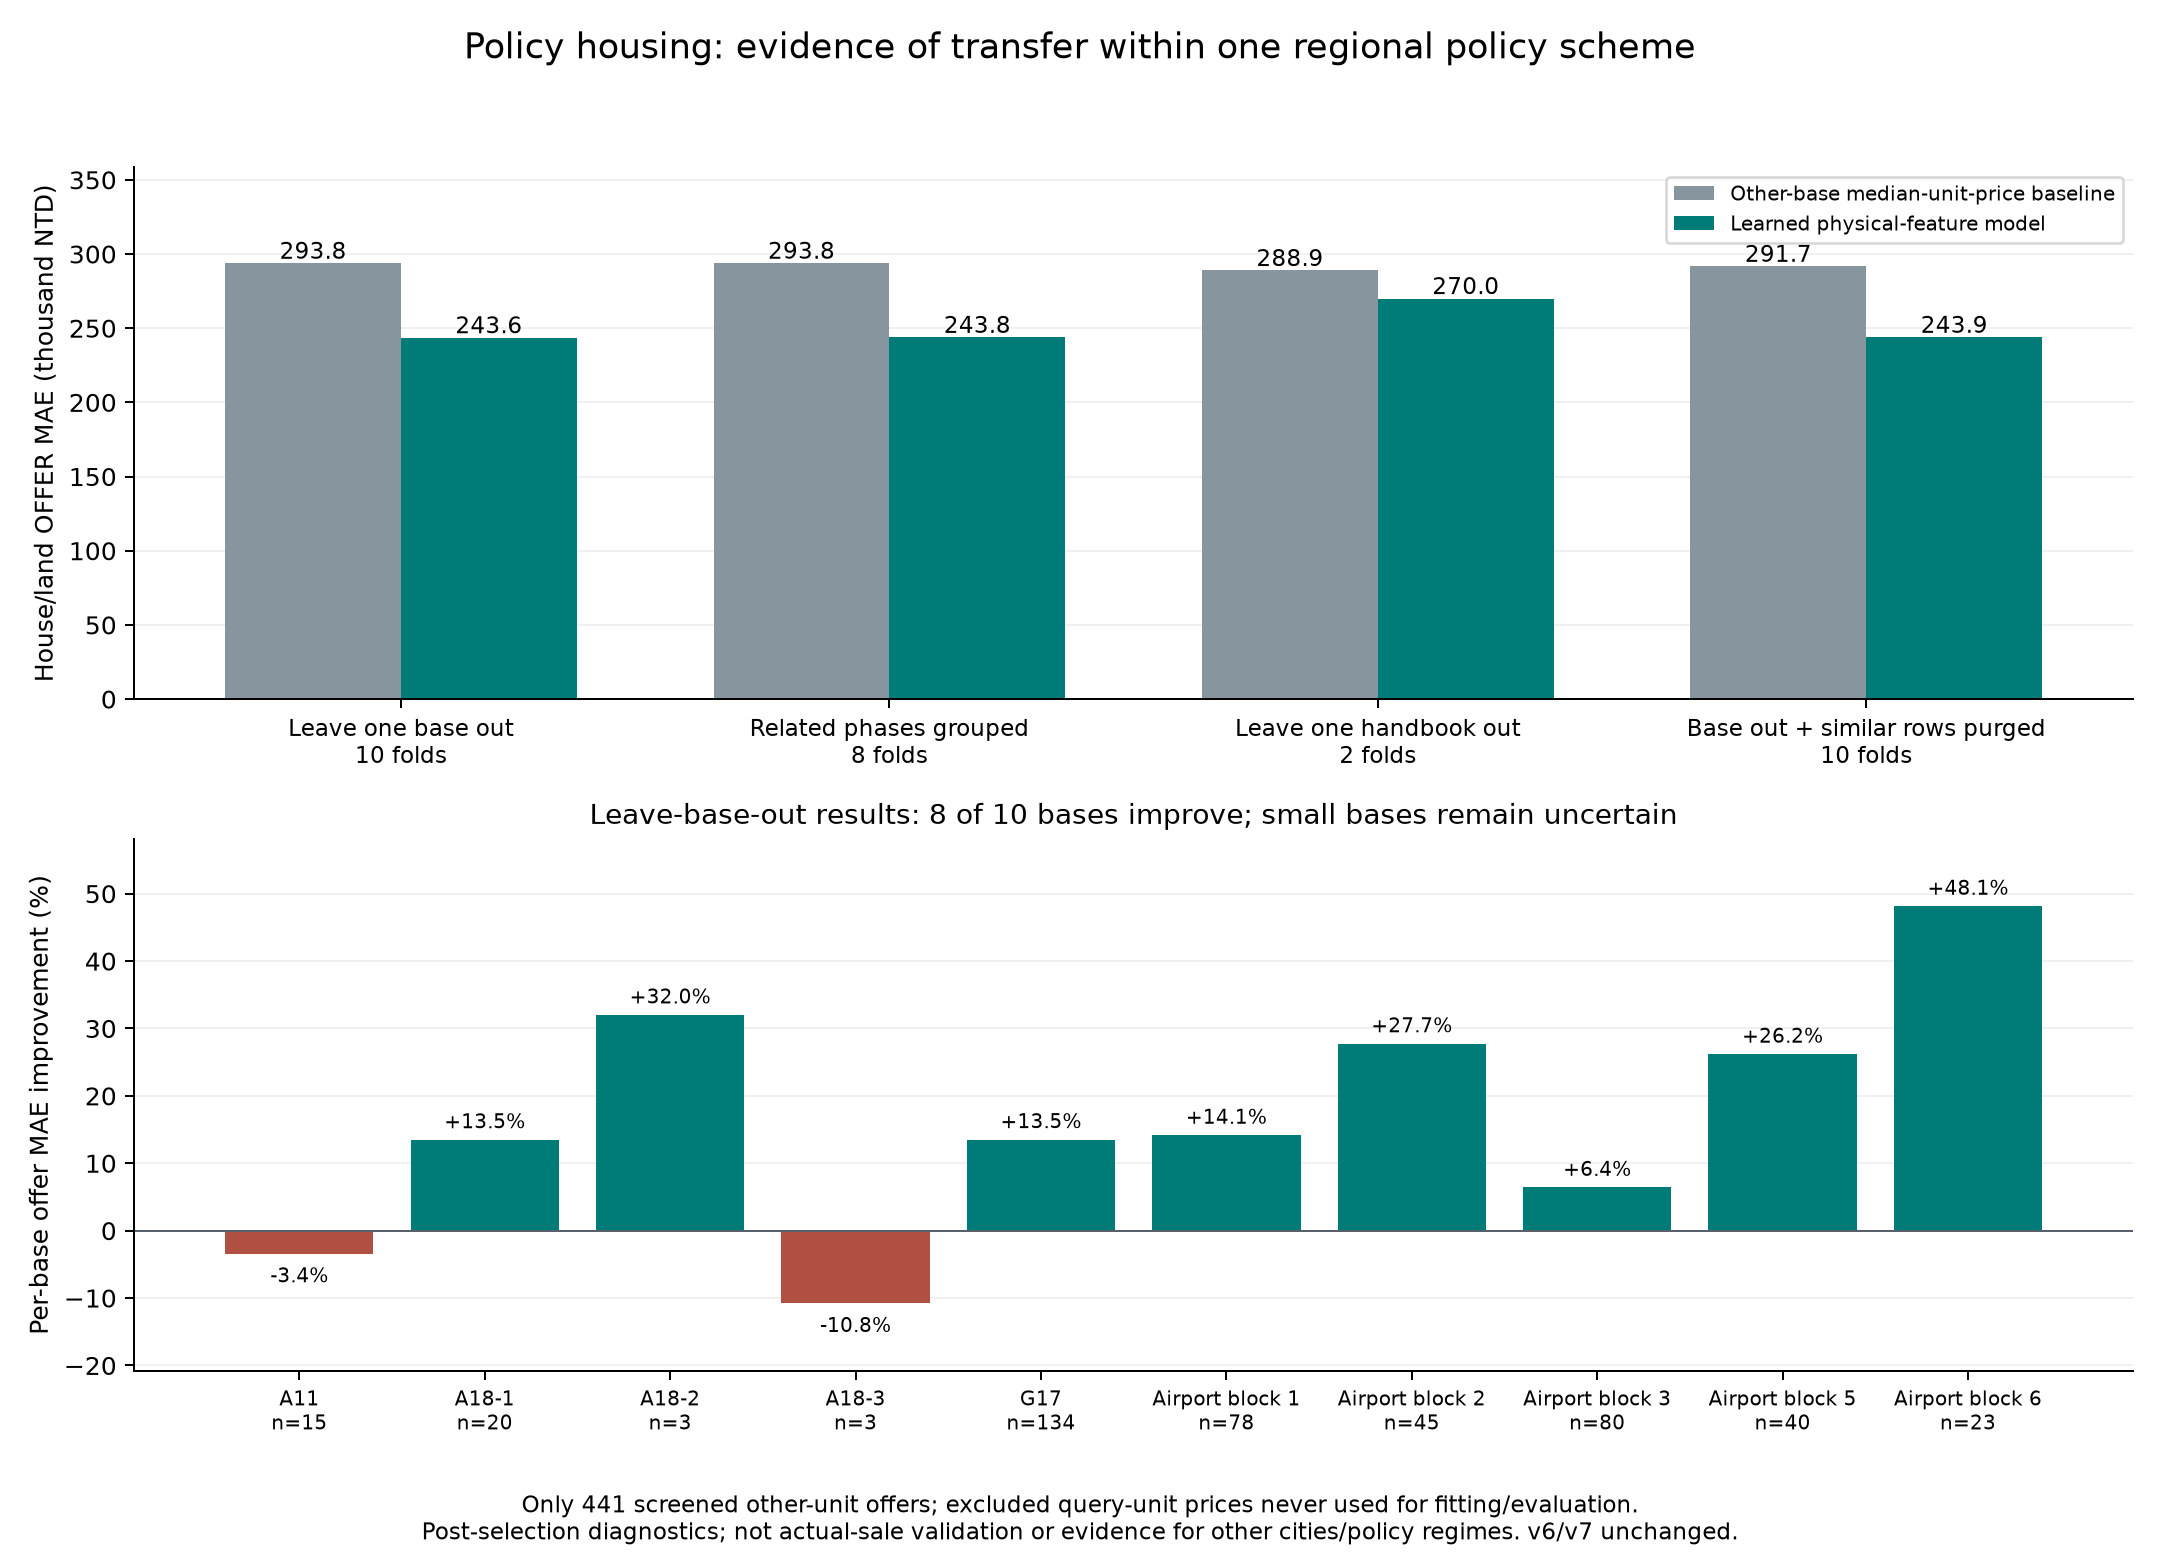
\includegraphics[width=.92\textwidth]{figures/policy_generalization.png}
\caption{同政策體系內跨基地測試。負結果與小基地樣本數均保留。}
\end{figure}

另外移除與任意 test 戶相似的 304 戶，只用剩餘 137 戶診斷重訓，房地預測變動中位數為 0.66\%、P95 為 2.41\%。
每筆查詢改用排除自身整基地的模型，變動中位數為 0.16\%、P95 為 1.80\%。
這些數字是穩定性檢查，沒有 test 目標，不能稱為 test 誤差。
二十次打亂訓練單價與特徵對應的負對照，MAE 均較差；因價格不具可交換性，不轉成正式顯著性 p 值。

結果支持\textbf{同一政策制度內的物理特徵學習與跨基地泛化}。
但跨來源改善的基地重抽樣區間包含零，兩份手冊也都屬桃園航空城，不能宣稱適用所有安置政策。
原 train 缺乏安置住宅成交標籤；報價與成交總價的差異仍未被直接驗證。

\section{外部資料時間、重現與限制}
地理來源 CSV 宣告提供日期為 2021-07-01，早於最早房價回測切點；目前下載檔案未獨立認證為當年原始快照。
政策手冊部分晚於 train 截止日，但早於受影響交易日期，不宣稱全部資訊在 2024-08-10 前已知。
外部資料使用依使用者限制進行，未取得完整官方競賽規則，因此不宣稱主辦方已認定合規。

本提交包包含原研究程式、聚合證據、來源雜湊、兩份最終候選與報告原始檔。
原始競賽資料、逐筆驗證標籤與約 4.5 GB 模型／快取不隨輕量 Git 包提供。
\texttt{scripts/verify\_package.py} 可在標準 Python 環境檢查包內檔案、CSV 格式及聚合數據一致性；
\texttt{project/} 中 46 項合成測試不需原始競賽資料。
完整推論重現另需還原資料、保存模型及外部來源快照，詳見 \texttt{REPRODUCIBILITY.txt}。

來源、設定、提交檔雜湊與推論重現紀錄可供追溯。
本報告整理與程式實作使用 AI 輔助；沒有以未實測的結果、隱藏 test 標籤或虛構 private 分數補足證據。
最終建議保留 v7 為主候選、v6 為備選，後續改進需以預先凍結方法與真正未查看的資料確認。

\begin{thebibliography}{9}
\bibitem{npa} 內政部警政署，歷史交通事故資料。
\url{https://data.gov.tw/dataset/12197}。使用的來源快照與雜湊保存在本專案證據包。
\bibitem{cawley} G. C. Cawley and N. L. C. Talbot.
On Over-fitting in Model Selection and Subsequent Selection Bias in Performance Evaluation.
Journal of Machine Learning Research, 11:2079--2107, 2010.
\url{https://www.jmlr.org/papers/v11/cawley10a.html}.
\bibitem{catboostfaq} CatBoost documentation, FAQ.
\url{https://catboost.ai/docs/en/concepts/faq}.
\bibitem{logo} scikit-learn documentation, LeaveOneGroupOut.
\url{https://scikit-learn.org/stable/modules/generated/sklearn.model_selection.LeaveOneGroupOut.html}.
\end{thebibliography}
\end{document}
